\documentclass[12pt]{article}
\usepackage{graphics,amssymb,amsmath}

\usepackage[slovak]{babel}
\usepackage[utf8]{inputenc}
\usepackage[IL2]{fontenc}

\usepackage{multicol}
\usepackage{mathtools}

\pagestyle{empty}
\setlength\textwidth{170mm}
\setlength\textheight{265mm}
\addtolength\oddsidemargin{-20mm}
\addtolength\topmargin{-20mm}
\setlength{\parindent}{1pt}
\setlength{\parskip}{10pt}
\newcount\pocet
\pocet = 1
\def\pr{{\bf \the \pocet .\ \global\advance\pocet by 1}}

\newcommand{\g}{ \dots \dots \dots \dots \dots \ }
\newcommand{\gu}{ \dots \dots \ }
\newcommand{\gr}{\dotfill \ }

\begin{document}

\newenvironment{itemize*}
 {\begin{itemize}
   \setlength{\itemsep}{0pt}
   \setlength{\parskip}{0pt}}
 {\end{itemize}}

\newenvironment{enumerate*}
 {\begin{enumerate}
   \setlength{\itemsep}{0pt}
   \setlength{\parskip}{0pt}}
 {\end{enumerate}}


\phantom{a}

\centerline{\textbf{\Large Matematika I}}
\smallskip
\centerline{08. jún 2018}
\centerline{08:00}
\vskip0.5cm

\centerline{\bf  Meno a priezvisko: \gr Podpis: \gr}
\vskip0.5cm
\centerline{\bf  Ročník: \gr Študijný program: \gr}
\vskip0.5cm

\medskip

\pr (7b) Daná je všeobecná rovnica kužeľosečky 
$9x^2-4y^2-1 = 0$.

\medskip

\noindent
\textbf{Doplňte:}
\begin{enumerate}
\item[a)] (2b) Kanonická rovnica (rovnica v štandardnom tvare) kužeľosečky je\gr
\item[b)] (1b) Typ kužeľosečky je \gr
\item[c)] (3b) Napíšte, ak existujú
\begin{itemize}
\item[$c_1$)] súradnice stredu kužeľosečky: \gr
\item[$c_2$)] súradnice ohniska resp. ohnísk kužeľosečky: \gr
\item[$c_3$)] súradnice vrcholu resp. vrcholov kužeľosečky: \gr
\end{itemize}
\item[d)] (1b) Znázornite kužeľosečku a v náčrte popíšte jej charakteristické prvky.
\end{enumerate}

\newpage

\pr (2b) Vyberte funkciu, ktorej definičný obor je znázornený na obrázku.
\begin{multicols}{2}
\noindent
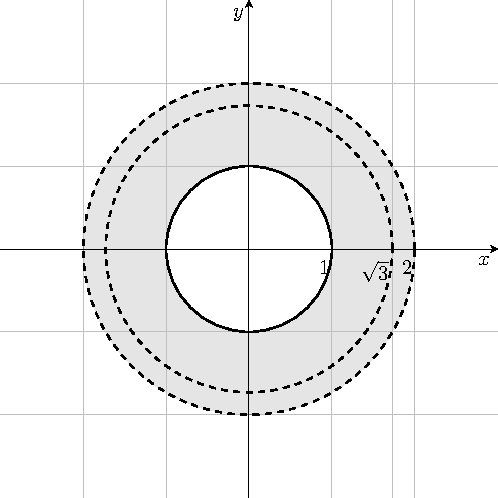
\includegraphics[width=6cm]{priklad5a.pdf}
\noindent
\begin{itemize}
\item[a)] $\displaystyle f(x,y)= \frac{\ln{(x^2+y^2-1)}}{\sqrt{4-x^2-y^2}}$
\item[b)] $\displaystyle f(x,y)= \frac{\sqrt{x^2+y^2-1}}{\ln{(4-x^2-y^2)}}$
\item[c)] $\displaystyle f(x,y)= \frac{\ln{(4-x^2-y^2)}}{\sqrt{x^2+y^2-1}}$
\item[d)] $\displaystyle f(x,y)= \frac{\sqrt{4-x^2-y^2}}{\ln(x^2+y^2-1)}$
\end{itemize}
\end{multicols}

\pr (6b) Vypočítajte 
$$\iint\limits_{M}{y} \ \mathrm{d}x \mathrm{d}y,$$ 
kde množina $M$ je mnohouholník s vrcholmi 
$A=[-1, -1]$, 
$B=[1, -1]$, 
$C=[4, 3]$,
$D=[-4, 3]$.

\begin{enumerate}
\item[]\textbf{Výsledok:}\gr
\end{enumerate}

\pr (4b) Bod $M$ má v cylindrickej súradnicovej sústave nasledujúce súradnice: $\displaystyle M=\left[\sqrt{2},\frac{3\pi}{4}, \sqrt{6}\right]$.

\begin{enumerate}
\item[a)] (2b) Vyberte správnu odpoveď:\\
Súradnice bodu $M$ v pravouhlej súradnicovej sústave sú:

\begin{multicols}{2}
\noindent
\begin{itemize}
\item[a)] $M=[1,-1,\sqrt{6}]$
\item[b)] $M=[-1,-1,\sqrt{6}]$
\end{itemize}

\noindent
\begin{itemize}
\item[c)] $M=[-1,1,\sqrt{6}]$
\item[d)] $M=[1,1,\sqrt{6}]$
\end{itemize}
\end{multicols}

\item[b)] (2b) Znázornite tento bod $M$ v pravouhlej súradnicovej sústave.

\begin{enumerate}
\item[]\textbf{Náčrt:}
\end{enumerate}
\end{enumerate}

\newpage

\bigskip

\pr (8b) Daná je lineárna obyčajná diferenciálna rovnica (LODR)
$y^{\prime\prime}(x) +6y^{\prime}(x)+9y(x) = x^2$.

\begin{enumerate}
\item[a)](2b) Napíšte charakteristickú rovnicu k danej diferenciálnej rovnici.
\medskip

\textbf{Charakteristická rovnica je:} \gr

\item[b)] (2b) Nájdite fundamentálny systém riešení diferenciálnej rovnice s nulovou pravou stranou.

\medskip

\textbf{Fundamentálny systém riešení je} \gr

\item[b)] (2b) Nájdite partikulárne riešenie uvedenej nehomogénnej rovnice.

\medskip

\textbf{Partikulárne riešene je} \gr

\item[c)] (2b) Napíšte všeobecné riešenie danej lineárnej diferenciálnej rovnice.

\medskip

\textbf{Všeobecné riešenie danej LODR je} \gr
\end{enumerate}

\bigskip

\pr (4b)
Vypočítajte, ak existuje

$$
\lim\limits_{
[x,y]\rightarrow [1,0]}
\frac{2-\sqrt{4-xy}}{xy}.
$$

\begin{enumerate}
\item[]\textbf{Výsledok:}\gr
\end{enumerate}


\pr (6b) Nájdite rovnicu dotykovej roviny $\tau$ ku grafu funkcie 
$\displaystyle f(x,y)=\dfrac{1}{x+y^2}$ \\ 
\hspace*{1.4cm} v bode $T=\left[x_{0},-1,\dfrac{1}{3}\right]$.

\begin{enumerate}
\item[] (2b) Nájdite $x_0$ a  \textbf{uveďte súradnice dotykového bodu}: \gr
\item[] (4b) \textbf{Rovnica} dotykovej roviny $\tau$ je:\gr
\end{enumerate}

\pr (6b) Daná je funkcia 
$\displaystyle f(x,y)=\ln(x+y)$, 
bod $\displaystyle A=[1, \, 2]$ 
a vektor $\displaystyle \vec{l}=\left(1, \, -2\right)$.

\begin{enumerate}
\item[a)] (3b) Nájdite gradient funkcie $f(x,y)$ v bode $A$.
\medskip

\textbf{Gradient} funkcie $f(x,y)$ v bode $A$ je \gr

\item[b)] (3b) Vypočítajte deriváciu funkcie $f(x,y)$ v bode $A$ v smere vektora $\vec{l}$.
\medskip

\textbf{Derivácia} funkcie $f(x,y)$ v bode $A$ v smere vektora $\vec{l}$ je \gr
\end{enumerate}

\newpage

\pr (27b) Daná je funkcia 
$f(x,y) = 1+9x^2+4y^2$ 
a oblasť $M$. \\
Oblasť $M$ je mnohouholník $ABCD$ s vrcholmi  
$A=[-2,-1]$, $B=[2,-1]$, $C=[4,1]$\linebreak  a $D=[-2,1]$.

\begin{enumerate}
\item[a)] Načrtnite oblasť $M$:

\textbf{Náčrt:}
\vspace{5cm}

\textbf{Pomocou matematických vzťahov popíšte hranice oblasti $M$:}
\begin{enumerate}
\item (2b) $AB$ \gr
\item (2b) $BC$ \gr
\item (2b) $CD$ \gr
\item (2b) $AD$ \gr
\end{enumerate}

\item[b)](5b) Nájdite lokálne extrémy danej funkcie $f(x, y)$ v oblasti $M$. \\
Ak hľadané lokálne extrémy nie sú, napíšte \uv{nie sú}.\\[1ex]
\hspace{5cm} \textbf{Doplňte odpoveď:}
Funkcia $f(x,y)$ má v bode \gr lokálne \gr
\medskip

\item[c)] Nájdite viazané lokálne extrémy danej funkcie $f(x, y)$ na hraniciach oblasti $M$.  
Ak hľadaný lokálny extrém nejestvuje, napíšte \uv{nie je}.

\begin{enumerate}
\item (3b) Na hranici $AB$ má funkcia $f(x,y)$  v bode \gr viazané lokálne \gr
\item (3b) Na hranici $BC$ má funkcia $f(x,y)$  v bode \gr viazané lokálne \gr
\item (3b) Na hranici $CD$ má funkcia $f(x,y)$  v bode \gr viazané lokálne \gr
\item (3b) Na hranici $AD$ má funkcia $f(x,y)$  v bode \gr viazané lokálne \gr
\end{enumerate}
\item[d)] (2b) Nájdite najväčšiu a najmenšiu hodnotu funkcie $f(x,y)$ na oblasti $M$.\\

\textbf{Najväčšia} hodnota funkcie $f(x,y)$ je: \gr

\textbf{Najmenšia} hodnota funkcie $f(x,y)$ je: \gr

\end{enumerate}

\end{document}
